% A LaTeX template for MSc Thesis submissions to 
% Politecnico di Milano (PoliMi) - School of Industrial and Information Engineering
%
% S. Bonetti, A. Gruttadauria, G. Mescolini, A. Zingaro
% e-mail: template-tesi-ingind@polimi.it
%
% Last Revision: October 2021
%
% Copyright 2021 Politecnico di Milano, Italy. NC-BY

\documentclass{Configuration_Files/PoliMi3i_thesis}

%------------------------------------------------------------------------------
%	REQUIRED PACKAGES AND  CONFIGURATIONS
%------------------------------------------------------------------------------

% CONFIGURATIONS
\usepackage{parskip} % For paragraph layout
\usepackage{setspace} % For using single or double spacing
\usepackage{emptypage} % To insert empty pages
\usepackage{multicol} % To write in multiple columns (executive summary)
\setlength\columnsep{15pt} % Column separation in executive summary
\setlength\parindent{0pt} % Indentation
\raggedbottom  

% PACKAGES FOR TITLES
\usepackage{titlesec}
% \titlespacing{\section}{left spacing}{before spacing}{after spacing}
\titlespacing{\section}{0pt}{3.3ex}{2ex}
\titlespacing{\subsection}{0pt}{3.3ex}{1.65ex}
\titlespacing{\subsubsection}{0pt}{3.3ex}{1ex}
\usepackage{color}

% PACKAGES FOR LANGUAGE AND FONT
\usepackage[english]{babel} % The document is in English  
\usepackage[utf8]{inputenc} % UTF8 encoding
\usepackage[T1]{fontenc} % Font encoding
\usepackage[10pt]{moresize} % Big fonts

% PACKAGES FOR IMAGES
\usepackage{graphicx}
\usepackage{transparent} % Enables transparent images
\usepackage{eso-pic} % For the background picture on the title page
\usepackage{subfig} % Numbered and caption subfigures using \subfloat.
\usepackage{tikz} % A package for high-quality hand-made figures.
\usetikzlibrary{}
\graphicspath{{./Images/}} % Directory of the images
\usepackage{caption} % Coloured captions
\usepackage{xcolor} % Coloured captions
\usepackage{amsthm,thmtools,xcolor} % Coloured "Theorem"
\usepackage{float}
\usepackage{tkz-euclide}

% STANDARD MATH PACKAGES
\usepackage{amsmath}
\usepackage{amsthm}
\usepackage{amssymb}
\usepackage{amsfonts}
\usepackage{bm}
\usepackage[overload]{empheq} % For braced-style systems of equations.
\usepackage{fix-cm} % To override original LaTeX restrictions on sizes

% PACKAGES FOR TABLES
\usepackage{tabularx}
\usepackage{longtable} % Tables that can span several pages
\usepackage{colortbl}

% PACKAGES FOR ALGORITHMS (PSEUDO-CODE)
\usepackage{algorithm}
\usepackage{algorithmic}

% PACKAGES FOR REFERENCES & BIBLIOGRAPHY
\usepackage[colorlinks=true,linkcolor=black,anchorcolor=black,citecolor=black,filecolor=black,menucolor=black,runcolor=black,urlcolor=black]{hyperref} % Adds clickable links at references
\usepackage{cleveref}
\usepackage[square, numbers, sort&compress]{natbib} % Square brackets, citing references with numbers, citations sorted by appearance in the text and compressed
\bibliographystyle{abbrvnat} % You may use a different style adapted to your field

% OTHER PACKAGES
\usepackage{pdfpages} % To include a pdf file
\usepackage{afterpage}
\usepackage{lipsum} % DUMMY PACKAGE
\usepackage{fancyhdr} % For the headers
\fancyhf{}

% Input of configuration file. Do not change config.tex file unless you really know what you are doing. 
\input{Configuration_Files/config}

%----------------------------------------------------------------------------
%	NEW COMMANDS DEFINED
%----------------------------------------------------------------------------

% EXAMPLES OF NEW COMMANDS
\newcommand{\bea}{\begin{eqnarray}} % Shortcut for equation arrays
\newcommand{\eea}{\end{eqnarray}}
\newcommand{\e}[1]{\times 10^{#1}}  % Powers of 10 notation

%----------------------------------------------------------------------------
%	ADD YOUR PACKAGES (be careful of package interaction)
%----------------------------------------------------------------------------

%----------------------------------------------------------------------------
%	ADD YOUR DEFINITIONS AND COMMANDS (be careful of existing commands)
%----------------------------------------------------------------------------

%----------------------------------------------------------------------------
%	BEGIN OF YOUR DOCUMENT
%----------------------------------------------------------------------------

\begin{document}

\fancypagestyle{plain}{%
\fancyhf{} % Clear all header and footer fields
\fancyhead[RO,RE]{\thepage} %RO=right odd, RE=right even
\renewcommand{\headrulewidth}{0pt}
\renewcommand{\footrulewidth}{0pt}}

%----------------------------------------------------------------------------
%	TITLE PAGE
%----------------------------------------------------------------------------

\pagestyle{empty} % No page numbers
\frontmatter % Use roman page numbering style (i, ii, iii, iv...) for the preamble pages

\puttitle{
	title=Topological Codes for Quantum Computation: the Toric Code, % Title of the thesis
	name=Alessia Conca Roncari, % Author Name and Surname
	course=Computer Science and Engineering - Ingegneria Informatica, % Study Programme (in Italian)
	ID  = 996809,  % Student ID number (numero di matricola)
	advisor= Prof. Michele Correggi, % Supervisor name
	coadvisor={Massimo Moscolari}, % Co-Supervisor name, remove this line if there is none
	academicyear={2023-24},  % Academic Year
} % These info will be put into your Title page 

%----------------------------------------------------------------------------
%	PREAMBLE PAGES: ABSTRACT (inglese e italiano), EXECUTIVE SUMMARY
%----------------------------------------------------------------------------
\startpreamble
\setcounter{page}{1} % Set page counter to 1

% ABSTRACT IN ENGLISH
\chapter*{Abstract} 
Here goes the Abstract in English of your thesis followed by a list of keywords.
The Abstract is a concise summary of the content of the thesis (single page of text)
and a guide to the most important contributions included in your thesis.
The Abstract is the very last thing you write.
It should be a self-contained text and should be clear to someone who hasn't (yet) read the whole manuscript.
The Abstract should contain the answers to the main scientific questions that have been addressed in your thesis.
It needs to summarize the adopted motivations and the adopted methodological approach as well as the findings of your work and their relevance and impact.
The Abstract is the part appearing in the record of your thesis inside POLITesi,
the Digital Archive of PhD and Master Theses (Laurea Magistrale) of Politecnico di Milano.
The Abstract will be followed by a list of four to six keywords.
Keywords are a tool to help indexers and search engines to find relevant documents.
To be relevant and effective, keywords must be chosen carefully.
They should represent the content of your work and be specific to your field or sub-field.
Keywords may be a single word or two to four words. 
\\
\\
\textbf{Keywords:} here, the keywords, of your thesis % Keywords

% ABSTRACT IN ITALIAN
\chapter*{Abstract in lingua italiana}
Qui va l'Abstract in lingua italiana della tesi seguito dalla lista di parole chiave.
\\
\\
\textbf{Parole chiave:} qui, vanno, le parole chiave, della tesi % Keywords (italian)

%----------------------------------------------------------------------------
%	LIST OF CONTENTS/FIGURES/TABLES/SYMBOLS
%----------------------------------------------------------------------------

% TABLE OF CONTENTS
\thispagestyle{empty}
\tableofcontents % Table of contents 
\thispagestyle{empty}
\cleardoublepage

%-------------------------------------------------------------------------
%	THESIS MAIN TEXT
%-------------------------------------------------------------------------
% In the main text of your thesis you can write the chapters in two different ways:
%
%(1) As presented in this template you can write:
%    \chapter{Title of the chapter}
%    *body of the chapter*
%
%(2) You can write your chapter in a separated .tex file and then include it in the main file with the following command:
%    \chapter{Title of the chapter}
%    \input{chapter_file.tex}
%
% Especially for long thesis, we recommend you the second option.

\addtocontents{toc}{\vspace{2em}} % Add a gap in the Contents, for aesthetics
\mainmatter % Begin numeric (1,2,3...) page numbering

% --------------------------------------------------------------------------
% NUMBERED CHAPTERS % Regular chapters following
% --------------------------------------------------------------------------
\chapter*{Introduction}

This document is intended to be both an example of the Polimi \LaTeX{} template for Master Theses,
as well as a short introduction to its use. It is not intended to be a general introduction to \LaTeX{} itself,
and the reader is assumed to be familiar with the basics of creating and compiling \LaTeX{} documents (see \cite{oetiker1995not, kottwitz2015latex}). 
\\
The cover page of the thesis must contain all the relevant information:
title of the thesis, name of the Study Programme and School, name of the author,
student ID number, name of the supervisor, name(s) of the co-supervisor(s) (if any), academic year.
The above information are provided by filling all the entries in the command \verb|\puttitle{}|
in the title page section of this template.
\\
Be sure to select a title that is meaningful.
It should contain important keywords to be identified by indexer.
Keep the title as concise as possible and comprehensible even to people who are not experts in your field.
The title has to be chosen at the end of your work so that it accurately captures the main subject of the manuscript. 
\\
Since a thesis might be a substantial document, it is convenient to break it into chapters.
You can create a new chapter as done in this template by simply using the following command
\begin{verbatim}
\chapter{Title of the chapter}
\end{verbatim}
followed by the body text.
\\
Especially for long manuscripts, it is recommended to give each chapter its own file.
In this case, you write your chapter in a separated \verb|chapter_n.tex| file
and then include it in the main file with the following command
\begin{verbatim}
\input{chapter_n.tex}
\end{verbatim}
It is recommended to give a label to each chapter by using the command
\begin{verbatim}
\label{ch:chapter_name}%
\end{verbatim}
where the argument is just a text string that you'll use to reference that part
as follows: \textit{Chapter~\ref{ch:chapter_one} contains \sc{an introduction to}  \dots}.\\
If necessary, an unnumbered chapter can be created by
\begin{verbatim}
\chapter*{Title of the unnumbered chapter}
\end{verbatim}






\chapter{Toric Code}
\label{ch:chapter_one}%
% The \label{...}% enables to remove the small indentation that is generated, always leave the % symbol.


\section{Description of the Model}
\label{sec:Model}

The Toric Code model is defined on a square lattice with periodic boundary conditions in both directions. These latter characteristics in topology are typical of what is known as a torus topology or simply a Torus, after which the model is named.\newline
A square lattice, here labelled as $L$, is a particular lattice defined in a two dimensional Euclidian space. It is denoted as $\mathbb{Z}^{2}$ such that each lattice point is identified with a tuple of integers. Though, the above mentioned boundary conditions also specify that for any point $(i, j)$ in the lattice, the neighboring points are going to be the following: $(i+1 \ mod \ L, j)$, $(i-1 \ mod \ L, j)$, $(i, j+1 \ mod \ L)$ and $(i, j-1 \ mod \ L)$.  \newline
Then, we are also going to consider a dual lattice, which will be labelled as $L'$, and that will be positioned as represented in figure 1.1, where the continuous line represents the main lattice $L$, while the dashed line represents its dual $L'$. 
On each edge is located a spin-$\frac{1}{2}$ particle, i.e. a Fermion, represented in the image below with an empty circle. Circles shaded in gray represent the boundaary conditions. \newline

\begin{figure}
\begin{center}
	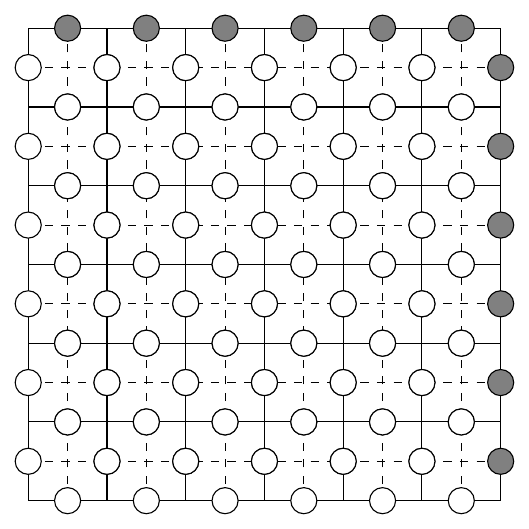
\begin{tikzpicture}
		% Draw dashed lines
		\foreach \i in {-3,-2.5,...,3}
		{
			\draw[dashed] (\i,-3) -- (\i,3);
		}
		\foreach \j in {-3,-2.5,...,3}
		{
			\draw[dashed] (-3,\j) -- (3,\j);
		}
		
		% Draw solid grid and nodes with circles in the middle of each side
		\draw[step=1cm] (-3,-3) grid (3,3);
		\foreach \i in {-2.5,...,2.5}
		{
			\foreach \j in {-2.5,...,2.5}
			{
				\begin{scope}[transform canvas={xshift=\i cm,yshift=\j cm}]
					\node[right,xshift=0.2cm,yshift=0.4cm] {};
					% Convert \j and \i to integers
					\pgfmathtruncatemacro{\intj}{\j}
					\pgfmathtruncatemacro{\inti}{\i}
					
					% Draw circles at the midpoints of each side
					\ifnum\intj=2
					\draw node[draw,circle,fill=gray] at (0,0.5) {};
					\else
					\draw node[draw,circle,fill=white] at (0,0.5) {};
					\fi
					
					\ifnum\inti=2
					\draw node[draw,circle,fill=gray] at (0.5,0) {};
					\else
					\draw node[draw,circle,fill=white] at (0.5,0) {};
					\fi
					
					\draw node[draw,circle,fill=white] at (0,-0.5) {};
					\draw node[draw,circle,fill=white] at (-0.5,0) {};
				\end{scope}
			}
		}
	\end{tikzpicture}
\end{center}

\caption{A square lattice with boundary conditions.}
\label{fig:lattice}
\end{figure}


For each cell on $L$ we are going to consider two spins, therefore the total number of spins will correspond to $2N$, where $N$ represents both the total number of cells in $L$ and the dimension of the lattice. 
Since all of these spins exhibit the same characteristics they are identified with identcial particles, which will be useful to know to study further properties of the model.

The key part of the model are the so called "vertex" and "plaquette" operators that are going to be placed, respectively, on the vertices $v$ and cells $p$ of $L$. Such operators can be defined formally as in definition 1.1.1 and implemented by means of Pauli matrices as exemplified in figure 1.2.
Throughout the description, the $Av$ operators are going to be shaded in blu, while the $Bp$ operators are going to be shaded in red. \newline

\textbf{Definition 1.1.1} (Vertex and Plaquette operators) Given a vertex $v$ and a plaquette $p$, we can define the following vertex and plaquette operators as tensor products over Pauli operators acting on four spins each located on the lattice and indicated by the indices $j \in star(v)$ and $j \in bdy(p)$  \newline 

\begin{center}
	$ Av = \prod_{j \in star(v)} Z_j $ \newline
	
	$ Bp = \prod_{j \in bdy(v)} X_j $.\newline
\end{center}



\begin{figure}
\begin{center}
	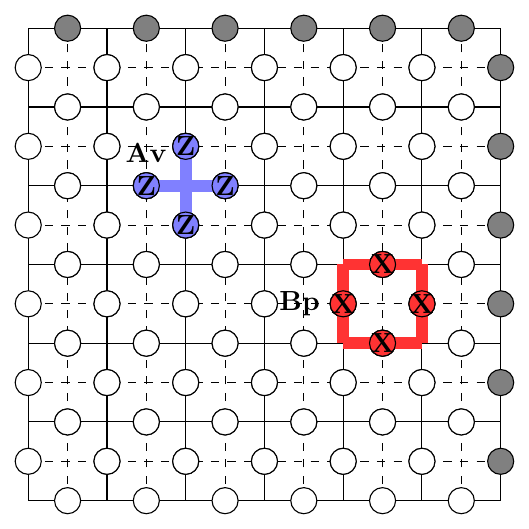
\begin{tikzpicture}
		% Draw dashed lines
		\foreach \i in {-3,-2.5,...,3}
		{
			\draw[dashed] (\i,-3) -- (\i,3);
		}
		\foreach \j in {-3,-2.5,...,3}
		{
			\draw[dashed] (-3,\j) -- (3,\j);
		}
		
		
		
		% Draw solid grid and nodes with circles in the middle of each side
		\draw[step=1cm] (-3,-3) grid (3,3);
		\foreach \i in {-2.5,...,2.5}
		{
			\foreach \j in {-2.5,...,2.5}
			{
				
				
				\begin{scope}[transform canvas={xshift=\i cm,yshift=\j cm}]
					\node[right,xshift=0.2cm,yshift=0.4cm] {};
					% Convert \j and \i to integers
					\pgfmathtruncatemacro{\intj}{\j}
					\pgfmathtruncatemacro{\inti}{\i}
					
					% Draw circles at the midpoints of each side
					\ifnum\intj=2
					\draw node[draw,circle,fill=gray] at (0,0.5) {};
					\else
					\draw node[draw,circle,fill=white] at (0,0.5) {};
					\fi
					
					\ifnum\inti=2
					\draw node[draw,circle,fill=gray] at (0.5,0) {};
					\else
					\draw node[draw,circle,fill=white] at (0.5,0) {};
					\fi
					
					\draw node[draw,circle,fill=white] at (0,-0.5) {};
					\draw node[draw,circle,fill=white] at (-0.5,0) {};
				\end{scope}
			}
		}
		
		\foreach \i in {-1,...,-1} %column
		{
			
			\draw[blue!50, line width=1.5mm] (\i,0.5) -- (\i,1.5);
			\node[draw, circle, fill=blue!50,label=center:\textbf{Z}] at (\i,0.5) {};
			\node[draw, circle, fill=blue!50,label=center:\textbf{Z}] at (\i,1.5) {};
			
		}
		\foreach \j in {1,...,1}
		{
			
			\draw[blue!50, line width=1.5mm] (-1.5, \j) -- (-0.5, \j);
			\draw node[draw,circle,fill=blue!50,label=center:\textbf{Z},,label=\textbf{Av}] at (-1.5,\j) {};
			\draw node[draw,circle,fill=blue!50,label=center:\textbf{Z}] at (-0.5,\j) {};
			
		}
		
		
		\foreach \i in {2,...,2}
		{
			
			\draw[red!80, line width=1.5mm] (\i,-1) -- (\i,0);
			\node[draw, circle, fill=red!80,label=center:\textbf{X}] at (\i,-0.5) {};
			
		}
		\foreach \j in {-1,...,-1}
		{
			
			\draw[red!80, line width=1.5mm] (2, \j) -- (1, \j);
			\draw node[draw,circle,fill=red!80,label=center:\textbf{X}] at (1.5,\j) {};
			
		}
		\foreach \i in {1,...,1}
		{
			
			\draw[red!80, line width=1.5mm] (\i,-1) -- (\i,0);
			\node[draw, circle, fill=red!80,label=center:\textbf{X},label=left:\textbf{Bp}] at (\i,-0.5) {};
			
		}
		\foreach \j in {0,...,0}
		{
			
			\draw[red!80, line width=1.5mm] (2, \j) -- (1, \j);
			\draw node[draw,circle,fill=red!80,label=center:\textbf{X}] at (1.5,\j) {};
			
		}
		
	\end{tikzpicture}
\end{center}
\caption{Veretx (red) and plaquette (blue) operators.}
\label{fig:operators}
\end{figure}


All the elements that constitute the model of the toric code are brought together by its Hamiltonian, which is given by the following definition:\newline

\textbf{Definition 1.1.2} (Toric Code Hamiltonian) Given sites $v$ and $p$ of the lattice along with their respective vertex and plaquette operators and given the spin-$\frac{1}{2}$ particles located on each edge of the torus, we can define the following Hamiltonian for the system:\newline

\begin{center}
	
	$H = -\sum_{v} 
	Av - \sum_{p} Bp $.\newline
	
\end{center}

Each one of the $Av$ and $Bp$ operators that appear in the Hamiltonian share some important properties, which are going to be covered in the following definitions and will later be used to further characterize the action of the operators. \newline


Firstly, notice that $Av$ and $Bp$ operators are Hermitian and square to the identity. \newline


\textbf{Definition 1.1.3} (Hermitian operator) Let $H$ be an Hilbert space and  $A$: $H \rightarrow H$ be a linear operator. An operator $A$ is called Hermitian if for all $\psi,\phi \in H$ we have that\newline

\begin{center}
	$\langle A\psi|\phi \rangle = \langle \psi|A^{\dagger}\phi \rangle = \langle \phi|A\psi \rangle^{*}$.
\end{center}

where the daga symbol $\dagger$ represents the conjugate transpose and the $\langle \ \rangle$ the Hermitian inner product. \newline
It is important for the following applications to specify that a square matrix $A$ of complex numbers, representing a linear operator, is called hermitian if $A^{\dagger} = (A^*)^T = A$. One important consequence of Hermiticity is that the corresponding eigenvalues of the operator are real. Note also that for real matrices, as in the case of our operators, it is sufficient to compute only the transpose of the matrix to verify hermiticity. \newline

Then, the involutory property comes from the unitarity of the matrices representing the vertex and plaquette operators, i.e. $X$ and $Z$ Pauli matrices. \newline

\textbf{Definition 1.1.4} (Unitary operator) Let $H$ be an Hilbert space. Let $U$: $H \rightarrow U$ be a linear operator. We define $U$ to be complex unitary if for all $\psi,\phi \in H$ we have that\newline

\begin{center}
	$\langle U\psi|U\phi \rangle = \langle \psi|\phi \rangle$.
\end{center}

In terms of the conjugate transpose, we can define a complex matrix $U$ to be unitary if $ (U^*)^T=U^{-1}$. We note that it is possible to define an operator to be real unitary, with the only difference that $(U)^T = U^{-1}$. Then, we can also define that a real matrix $U$, representing a linear operator, is unitary if $(U)^T = U^{-1}$ or, equivalently, if $(U)^T U=I$. Note also that one important property of  unitary operators is that their eigenvalues have modulus equal to one.\newline

Given the considerations made in Definition 1.1.3. and 1.1.4. for ral matrices, we can easily prove the first following proposition: \newline


\textbf{Proposition 1.1.1} (Hermiticity and involutory property of $Av$ and $Bp$ operators)
$Av$ and $Bp$ operators are Hermitian and satisfy the involutory property.\newline

\textit{Proof.}\newline

We know that the operator $ Av = \prod_{j \in star(v)} Z_j $ and that $ Bp = \prod_{j \in bdy(v)} X_j $ .\newline

Firstly, recall the form of the $\sigma_x$ and $\sigma_z$ matrices representing the Pauli gates $X$ and $Z$:



\[
\text{Z = $\sigma_z$} =
\begin{bmatrix}
	1 & 0 \\
	0 & -1
\end{bmatrix}
\]


\[
\text{X = $\sigma_x$} =
\begin{bmatrix}
	0 & 1 \\
	1 & 0
\end{bmatrix}
\]


	Prove that they are Hermitian:\newline

\[
\text{$( \sigma_z )^{H}$} = 
\begin{bmatrix}
	1 & 0 \\
	0 & -1
\end{bmatrix} ^H =
\begin{bmatrix}
	1 & 0 \\
	0 & -1
\end{bmatrix}^T =
\begin{bmatrix}
	1 & 0 \\
	0 & -1
\end{bmatrix}
= \text{$ \sigma_z $}
\]


\[
\text{$( \sigma_x )^{H}$} = 
\begin{bmatrix}
	0 & 1 \\
	1 & 0
\end{bmatrix} ^H =
\begin{bmatrix}
	0 & 1 \\
	1 & 0
\end{bmatrix}^T =
\begin{bmatrix}
	0 & 1 \\
	1 & 0
\end{bmatrix}
= \text{$ \sigma_x $}
\]\newline

Note that Pauli matrices are real matrices, i.e. $A^{\dagger}=A^T$.
Then, knowing that $[\sigma_i,\sigma_j]=0 \ for \ i=j$ we can write		\newline

\begin{center}
	$(Av)^{\dagger} = (\sigma_{x_1} \sigma_{x_2} \sigma_{x_3} \sigma_{x_4})^{\dagger} = \sigma_{x_1}^{\dagger} \sigma_{x_2}^{\dagger} \sigma_{x_3}^{\dagger} \sigma_{x_4}^{\dagger} = \sigma_{x_1} \sigma_{x_2} \sigma_{x_3} \sigma_{x_4} = Av$ \newline
	
	$(Bp)^{\dagger} = (\sigma_{z_1} \sigma_{z_2} \sigma_{z_3} \sigma_{z_4})^{\dagger} = \sigma_{z_1}^{\dagger} \sigma_{z_2}^{\dagger} \sigma_{z_3}^{\dagger} \sigma_{z_4}^{\dagger} = \sigma_{z_1} \sigma_{z_2} \sigma_{z_3} \sigma_{z_4} = Bp$\newline
\end{center}

Prove the involutory propertyy:\newline

\[
\text{$( \sigma_z )^{2}$} = 
\begin{bmatrix}
	1 & 0 \\
	0 & -1
\end{bmatrix} *
\begin{bmatrix}
	1 & 0 \\
	0 & -1
\end{bmatrix} =
\begin{bmatrix}
	1 & 0 \\
	0 & 1
\end{bmatrix}
= \text{$I$}
\]


\[
\text{$( \sigma_x )^{2}$} = 
\begin{bmatrix}
	0 & 1 \\
	1 & 0
\end{bmatrix} *
\begin{bmatrix}
	0 & 1 \\
	1 & 0
\end{bmatrix} =
\begin{bmatrix}
	1 & 0 \\
	0 & 1
\end{bmatrix}
= \text{$I$}
\]\newline


Then, again we can write\newline

\begin{center}
	$(Av)^{2} = (\sigma_{x_1} \sigma_{x_2} \sigma_{x_3} \sigma_{x_4})^{2} = \sigma_{x_1}^2 \sigma_{x_2}^2 \sigma_{x_3}^2 \sigma_{x_4}^2 = I$ \newline
	
	$(Bp)^{2} = (\sigma_{z_1} \sigma_{z_2} \sigma_{z_3} \sigma_{z_4})^{2} = \sigma_{z_1}^2 \sigma_{z_2}^2 \sigma_{z_3}^2 \sigma_{z_4}^2 = I$\newline
\end{center}

\hfill $\square$\newline

	Given Proposition 1.1.1, we can know further characterize the opeartors in terms of their eigenvalues and define their spectrum.	\newline

\textbf{Proposition 1.1.2} (Eigenvalues of $Av$ and $Bp$ operators) Given Hermitian operators $Av$ and $Bp$, which satisfying the involutory property, their eigenvalues are $\pm 1$.
\newline

\textit{Proof.}\newline

Given the Hermiticity and involutory proof in 1.1.1, we firstly prove that Hermitian operators (and therefore our vertex and plaquette operators) have real eigenvalues: \newline

Write the expression for the eigenvalues $Av |\xi \rangle = \lambda |\xi \rangle$ and take as hypothesis that $|\xi \rangle \neq 0$. Then, by means of the scalar product\newline

\begin{center}
	$\langle \xi|Av|\xi \rangle = \lambda \langle \xi | \xi \rangle$\newline
	
	$\lambda = \frac {\langle \xi|Av|\xi \rangle}{\langle \xi |\xi \langle}$ = $\frac {\langle \xi|Av|\xi \rangle}{||\xi||^2}$ = $\frac {\langle \xi|Av^{\dagger}|\xi \rangle}{||\xi||^2}$ = $\frac {\langle \xi|Av|\xi\rangle^*}{||\xi||^2}$ = $\lambda^*$\newline
\end{center}

Notice that we have applied antilinearity of the adjoint in the penultimate equality: \newline

\begin{center}
	$(\langle \xi|Av^{\dagger}|\xi \rangle)^{\dagger}$ = $|\xi\rangle^{\dagger} (Av^{\dagger})^{\dagger} \langle\xi|^{\dagger}$ = $\langle \xi|Av|\xi \rangle^*$. \newline
\end{center}

Using hermiticity with the fact that $(Av)^2=I$ we can derive the unitarity of $Av$ and state that $Av Av^{\dagger} = Av^{\dagger} Av = (Av)^2 = I$, i.e. for a unitary operator $U$ we have $U^{\dagger}=U^{-1}$. \newline

Given the property of unitary operators that states that their eigenvalues have modulus equal to one:\newline 


By taking as hypothesis $|\xi \rangle \neq 0$, we write the expression $U |\xi \rangle = \lambda |\xi \rangle$ and its self-adjoint $\langle \xi| U^{\dagger} = \lambda^* \langle \xi|$. Then, knowing that $U^{\dagger}=U^{-1}$, by means of the scalar product we obtain \newline

\begin{center}
	$\langle \xi|U U^{\dagger}|\xi\rangle = \lambda \lambda^* \langle \xi |\xi \rangle$\newline
	
	$\langle \xi|I|\xi \rangle = \lambda \lambda^* \langle \xi |\xi \rangle$\newline
	
	$\langle \xi|\xi \rangle = \lambda \lambda^* \langle \xi |\xi \rangle $\newline
\end{center}

Finally, since we already know that Hermitian operators have real eigenvalues we can write $|\lambda|^2 = 1$.\newline

Putting together the fact that $Av$ has real eigenvalues with unitarity we obtain that the only two remaining possibilities for the eigenvalues of $Av$ are $\pm 1$. \newline


The same reasoning can be carried out for the $Bp$ operator.

\hfill $\square$ \newline

Given the result of proposition 1.1.2, the spectrum of the operators is easy to find:	\newline

\textbf{Proposition 1.1.3} (Spectrum of $Av$ and $Bp$ operators) The spectrum of $Av$ and $Bp$ operators is equal to $ \{-1,+1\}$. \newline

We now analyze the relationship between vertex and plaquette operators. Such relationship is characterized by two fundamental mathematical concepts called "commutation" and "anticommutation". These relations serve as an important result in understanding the stability and fault-tolerance of the toric code.	\newline

\textbf{Proposition 1.1.4} (Commutation of $Av$ and $Bp$ operators) The operator Av commutes with the operator Bp for an even number of edges.
\newline

\textbf{Proposition 1.1.5} (Anticommutation of $Av$ and $Bp$ operators) The operator $Av$ anticommutes with the operator $Bp$ for an odd number of edges.
\newline

\textit{Proof.}\newline 
%Av commutes with itself.\newline
%Bp commutes with itself.\newline
%Av commutes with Bp for an even number of edges.\newline

Fix the origin of the coordinate system in the bottom left corner of the lattice as indicated in the picture below:\newline

%picture

then, we can define the two vectors representing the site of application of the vertex and plaquette operator, respectively over the lattice L and dual lattice L'

\begin{center}
	$\vec{v}$= $n\hat{e_1} + m\hat{e_2}$, where $n,m \in \mathbb{Z}$ \newline
	
	$\vec{p}$= $(n + \frac{1}{2}) \hat{e_1} + (m + \frac{1}{2}) \hat{e_2}$, where $n,m \in \mathbb{Z}$\newline
\end{center}

Rewrite the operators as follows:\newline

\begin{center}
	
	$A_{\vec{v}} = \sigma^z_{\vec{v}+\frac{1}{2}\hat{e_1}} \sigma^z_{\vec{v}+\frac{1}{2}\hat{e_2}} \sigma^z_{\vec{v}-\frac{1}{2}\hat{e_1}} \sigma^z_{\vec{v}-\frac{1}{2}\hat{e_2}}$ \newline
	
	$B_{\vec{p}} = \sigma^x_{\vec{p}+\frac{1}{2}\hat{e_1}} \sigma^x_{\vec{p}+\frac{1}{2}\hat{e_2}} \sigma^x_{\vec{p}-\frac{1}{2}\hat{e_1}} \sigma^x_{\vec{p}-\frac{1}{2}\hat{e_2}}$\newline
	
\end{center}

In order to simplify the calculations we rewrite $Bp$ on the lattice L by rewriting the indeces in terms of vector $\vec{v}$

\begin{center}
	$(n\hat{e_1} + m\hat{e_2}) + \frac{1}{2}\hat{e_2}= n\hat{e_1} + (m+\frac{1}{2}\hat{e_2})$\newline
	
	$(n\hat{e_1} + m\hat{e_2}) + \frac{1}{2}\hat{e_1}= (n+ \frac{1}{2})\hat{e_1} + m\hat{e_2}$\newline
	
	$(n\hat{e_1} + m\hat{e_2}) + \frac{1}{2}\hat{e_1}+\hat{e_2}= (n+ \frac{1}{2})\hat{e_1} + (m + 1)\hat{e_2}$\newline
	
	$(n\hat{e_1} + m\hat{e_2}) + \frac{1}{2}\hat{e_2}+\hat{e_1}= (n+ 1)\hat{e_1} + (m + \frac{1}{2})\hat{e_2}$\newline
\end{center}


Then the $B_{\vec{p}}$ operator becomes:

\begin{center}
	
	$B_{\vec{v}} = \sigma^x_{n\hat{e_1} + (m+\frac{1}{2}\hat{e_2})} \sigma^x_{(n+ \frac{1}{2})\hat{e_1} + m\hat{e_2}} \sigma^x_{(n+ \frac{1}{2})\hat{e_1} + (m + 1)\hat{e_2}} \sigma^x_{(n+ 1)\hat{e_1} + (m + \frac{1}{2})\hat{e_2}}$\newline
	
\end{center}



and the Hamiltonian can be written by grouping the indices:\newline

\begin{center}
	
	$H = - \sum_{m,n \in \mathbb{Z}} \{ 
	\sigma^z_{(n+\frac{1}{2})\hat{e_1} + m\hat{e_2}} \sigma^z_{n\hat{e_1}+(m+\frac{1}{2})\hat{e_2}} \sigma^z_{(n-\frac{1}{2})\hat{e_1} + m\hat{e_2}} \sigma^z_{n\hat{e_1}+(m-\frac{1}{2})\hat{e_2}} +
	\sigma^x_{n\hat{e_1} + (m+\frac{1}{2}\hat{e_2})} \sigma^x_{(n+ \frac{1}{2})\hat{e_1} + m\hat{e_2}} \sigma^x_{(n+ \frac{1}{2})\hat{e_1} + (m + 1)\hat{e_2}} \sigma^x_{(n+ 1)\hat{e_1} + (m + \frac{1}{2})\hat{e_2}} \} $
	
\end{center}

Now calcuate the commutator $[A_{\vec{v}},B_{\vec{v}}] = A_{\vec{v}}B_{\vec{v}} - B_{\vec{v}}A_{\vec{v}}$ by focusiing on the first term:\newline

\begin{center}
	
	$ A_{\vec{v}}B_{\vec{v}} =
	\sigma^z_{(n+\frac{1}{2})\hat{e_1} + m\hat{e_2}} \sigma^z_{n\hat{e_1}+(m+\frac{1}{2})\hat{e_2}} \sigma^z_{(n-\frac{1}{2})\hat{e_1} + m\hat{e_2}} \sigma^z_{n\hat{e_1}+(m-\frac{1}{2})\hat{e_2}} $ *
	
	$\sigma^x_{n\hat{e_1} + (m+\frac{1}{2}\hat{e_2})} \sigma^x_{(n+ \frac{1}{2})\hat{e_1} + m\hat{e_2}} \sigma^x_{(n+ \frac{1}{2})\hat{e_1} + (m + 1)\hat{e_2}} \sigma^x_{(n+ 1)\hat{e_1} + (m + \frac{1}{2})\hat{e_2}}$\newline
	
\end{center}


Matrices do not commute but for Pauli matrices we have the following commutation relationship :\newline


\begin{center}
	$\sigma^x_{\vec{v}}\sigma^z_{\vec{v}'} = \sigma^z_{\vec{v}'} \sigma^x_{\vec{v}} + 2* \sigma^x_{\vec{v}}\sigma^z_{\vec{v}'} \delta_{\vec{v} \vec{v}'}$\newline
\end{center}


where $\hspace{1cm} \delta_{\vec{v} \vec{v}'} =$
$\begin{cases}
	1, \hspace{1cm} if \hspace{1cm}  \vec{v} = \vec{v}'\\
	0, \hspace{1cm} if \hspace{1cm} \vec{v} \neq \vec{v}'
\end{cases}$\newline

which states that 	$\sigma^x_{\vec{v}}\sigma^z_{\vec{v}'}$ commutate for $\vec{v} \neq \vec{v}'$   but anticommutate for $\vec{v} = \vec{v}'$. This is known from the anticommutation relationship of Pauli matrices $\sigma^x \sigma^z = - \sigma^x \sigma^z$. Thus, for an even numer of overlapping edges, in our case 2 or 4, the commutator becomes:\newline

\begin{center}
	
	$[A_{\vec{v}},B_{\vec{v}}] = 2 *
	\sigma^x_{n\hat{e_1} + (m+\frac{1}{2}\hat{e_2})} \sigma^x_{(n+ \frac{1}{2})\hat{e_1} + m\hat{e_2}} \sigma^x_{(n+ \frac{1}{2})\hat{e_1} + (m + 1)\hat{e_2}} \sigma^x_{(n+ 1)\hat{e_1} + (m + \frac{1}{2})\hat{e_2}}*
	\sigma^z_{(n+\frac{1}{2})\hat{e_1} + m\hat{e_2}} \sigma^z_{n\hat{e_1}+(m+\frac{1}{2})\hat{e_2}} \sigma^z_{(n-\frac{1}{2})\hat{e_1} + m\hat{e_2}} \sigma^z_{n\hat{e_1}+(m-\frac{1}{2})\hat{e_2}} $ 	\newline 
	
	
\end{center}
Instead, for an odd number of edges it becomes null $[A_{\vec{v}},B_{\vec{v}}]=0$.\newline

This calculations conclude that $A_{\vec{v}},B_{\vec{p}}$ commute for an even numer of edges but anticommute for an odd number of edges.\newline

\hfill $\square$\newline



%--------------



\section{Ground State}
\label{sec:GS}




\section{Excited States}
\label{sec:ES}




\section{Anyonic Excitations}
\label{sec:AE}











\chapter{Coding on the Toric Code}
\label{ch:chapter_two}

\section{Classical Error Correction}
\label{sec:CER}



\section{Quantum Error Correction (QEC)}
\label{sec:QEC}



\section{QEC in the Toric Code}
\label{sec:TC}













\chapter{Conclusions and future developments}
\label{ch:conclusions}%
A final chapter containing the main conclusions of your research/study
and possible future developments of your work have to be inserted in this chapter.

%-------------------------------------------------------------------------
%	BIBLIOGRAPHY
%-------------------------------------------------------------------------

\addtocontents{toc}{\vspace{2em}} % Add a gap in the Contents, for aesthetics
\bibliography{Thesis_bibliography} % The references information are stored in the file named "Thesis_bibliography.bib"

%-------------------------------------------------------------------------
%	APPENDICES
%-------------------------------------------------------------------------

\cleardoublepage
\addtocontents{toc}{\vspace{2em}} % Add a gap in the Contents, for aesthetics







% LIST OF FIGURES
\listoffigures

% LIST OF SYMBOLS
% Write out the List of Symbols in this page
\chapter*{List of Symbols} % You have to include a chapter for your list of symbols (
\begin{table}[H]
    \centering
    \begin{tabular}{lll}
        \textbf{Variable} & \textbf{Description} & \textbf{SI unit} \\\hline\\[-9px]
        $\bm{u}$ & solid displacement & m \\[2px]
        $\bm{u}_f$ & fluid displacement & m \\[2px]
    \end{tabular}
\end{table}




% ACKNOWLEDGEMENTS
\chapter*{Acknowledgements}
Here you might want to acknowledge someone.

\cleardoublepage

\end{document}
